% !TeX root = construct.tex

\chapter{A Straightedge (with Something Extra) is Sufficient}\label{c.straightedge}

Can every construction with straightedge and compass be done with only a straightedge? The answer is no. In 1822 the French mathematician Jean-Victor Poncelet conjectured that a straightedge only is sufficient, provided that one circle exists in the plane. This theorem was proved in 1833 by the Swiss mathematician Jakob Steiner. In this chapter I present a proof of the theorem based on the one appearing as problem 34 in \cite{dorrie1} as reworked by Michael Woltermann \cite{dorrie2}.\footnote{I would like to thank him for giving me permission to use his work.}

Every step of a construction with straightedge and compass can is one of the following three operations:
\begin{itemize}
\setlength{\itemsep}{0pt}
\item Finding the point of intersection of two straight lines.
\item Finding the point(s) of intersection of a straight line and a circle.
\item Finding the point(s) of intersection of two circles.
\end{itemize}
It is clear that the first operation can be performed with a straightedge only. For the other two operations, we have to find an equivalent construction with straightedge alone.

What does it mean to perform a construction with straight-edge alone? A circle is defined by a point $O$, its center, and a line segment whose length is the radius $r$, one of whose endpoints is the center. If we can construct the points $X,Y$ labeled in the following diagram, we can claim to have successfully constructed the intersection of a given circle with a given line and of two given circles. The circles drawn with dashed lines in the diagram do not actually appear in the construction. In this chapter, the single existing circle is drawn with a regular line, and the dashed circles are only used to help understand a construction and its proof.
\begin{center}
\begin{tikzpicture}[scale=.9]
\fill (0,0) node[above right] {$O$} circle[radius=1.5pt];
\draw[thick,dashed,name path=circle] (0,0) circle[radius=2cm];
\draw (0,0) -- node[left] {$r$} ++(-60:2cm);
\fill (0,0) ++(-60:2cm) circle[radius=1.5pt];
\draw[name path=line] (-3,-.5) -- ++(20:6cm);
\path [name intersections={of=circle and line,by={X,Y}}];
\fill (X) node[above right,xshift=-2pt,yshift=4pt] {$X$} circle[radius=1.5pt];
\fill (Y) node[above left] {$Y$} circle[radius=1.5pt];
\begin{scope}[xshift=6cm]
\fill (0,0) node[above right] {$O_1$} circle[radius=1.5pt];
\fill (3,0) node[above right] {$O_2$} circle[radius=1.5pt];
\draw[thick,dashed,name path=circle1] (0,0) circle[radius=2cm];
\draw[thick,dashed,name path=circle2] (3,0) circle[radius=2cm];
\draw (0,0) -- node[left] {$r_1$} ++(-60:2cm);
\draw (3,0) -- node[left,below] {$r_2$} ++(-20:2cm);
\fill (3,0) ++(-20:2cm) circle[radius=1.5pt];
\path [name intersections={of=circle1 and circle2,by={X,Y}}];
\fill (X) node[above,yshift=4pt] {$X$} circle[radius=1.5pt];
\fill (Y) node[below,yshift=-4pt] {$Y$} circle[radius=1.5pt];
\end{scope}
\end{tikzpicture}
\end{center}

First we present five necessary auxiliary constructions (Sections~\ref{s.parallel}--\ref{s.root}), and then show how to find the intersection of a line with a circle (Section~\ref{s.line-circle-straight}) and of two circles (Section~\ref{s.two-circles}).

\newpage

\section{Constructing a line parallel to a given line}\label{s.parallel}

\textbf{Given a line $l$ defined by two points $A,B$ and a point $P$ not on the line, it is possible to construct a line through $P$ that is parallel to $AB$.}

There are two cases:
\begin{itemize}
\setlength{\itemsep}{0pt}
\item A ``directed line'': The midpoint $M$ of $AB$ is given.
\item Any other line.
\end{itemize}

\textbf{Case 1, directed line}: Construct a ray that extends $AP$ and choose any point $S$ on the ray beyond $P$. Construct the line $BP,SM,SB$. Label by $O$ the intersection of $BP$ with $SM$. Construct a ray that extends $AO$ and label by $Q$ the intersection of the ray $AO$ with $SB$.

\begin{center}
\vspace*{-8pt}
\begin{tikzpicture}
\draw[name path=pq] (-4,0) -- (4,0);
\draw (-2,-2) node[below left] {$A$} coordinate (A) -- (2,-2) node[below right] {$B$} coordinate (B);
\fill (A) circle[radius=1.5pt];
\fill (B) circle[radius=1.5pt];
\draw[name path=as] (A) -- ++(50:4cm) node[above] {$S$} coordinate (S);
\fill (S) circle[radius=1.5pt];
\draw[name path=sb] (S) -- (B);
\path [name intersections={of=pq and as,by={P}}];
\path [name intersections={of=pq and sb,by={Q}}];
\fill (P) node[above left] {$P$} circle[radius=1.5pt];
\fill (Q) node[above right] {$Q$} circle[radius=1.5pt];
\draw[name path=pb] (P) -- (B);
\draw[name path=qa] (Q) -- (A);
\path [name intersections={of=pb and qa,by={O}}];
\fill (O) node[right,xshift=2pt] {$O$} circle[radius=1.5pt];
\fill (0,-2) coordinate (M) node[below right] {$M$} circle[radius=1.5pt];
\draw (S) -- (M);
\end{tikzpicture}
\vspace*{-6pt}
\end{center}

\textbf{$PQ$ is parallel to $AB$.}

\textbf{Proof:} We will use Ceva's theorem that we proof later.

\textbf{Theorem (Ceva):} Given three line segments from the vertices of a triangle to the opposite edges that intersect in a point (as in the diagram, but $M$ is not necessarily the midpoint of the side), the lengths of the segments satisfy:
\[
\frac{AM}{MB}\cdot\frac{BQ}{QS}\cdot\frac{SP}{PA} = 1\,.
\]

In the construction above, $M$ is the midpoint of $AB$, so $\disfrac{AM}{MB}=1$. The first factor in the multiplication cancels and we get the equation:
\begin{equation}
\frac{BQ}{QS}=\frac{PA}{SP}=\frac{AP}{PS}\,.\label{eq.ceva}
\end{equation}
We will prove that $\triangle ABS \sim \triangle PQS$, so that $PQ$ is parallel to $AB$ because $\angle ABS = \angle PQS$). The proof is as follows:
\erh{12pt}
\begin{equationarray*}{rcl}
BS&=&BQ+QS\\
\disfrac{BS}{QS}&=&\disfrac{BQ}{QS}+\disfrac{QS}{QS} = \disfrac{BQ}{QS}+1\\
AS&=&AP+PS\\
\disfrac{AS}{PS} &=& \disfrac{AP}{PS} + \disfrac{PS}{PS} = \disfrac{AP}{PS} + 1\\
\disfrac{BS}{QS}&=&\disfrac{BQ}{QS}+1=\disfrac{AP}{PS}+1=\disfrac{AS}{PS}\,,
\end{equationarray*}
where the last equation is obtained from Equation~\ref{eq.ceva}.

\textbf{Proof of Ceva's theorem:} Examine the following diagrams:

\vspace{-4ex}

\begin{center}
\begin{tikzpicture}
\path[name path=pq] (-4,0) -- (4,0);
\draw (-2,-2) node[below left] {$A$} coordinate (A) -- (2,-2) node[below right] {$B$} coordinate (B);
\coordinate (M) at (0,-2);
\draw[name path=as] (A) -- ++(50:4cm) node[above] {$S$} coordinate (S);
\draw[name path=sb] (S) -- (B);
\path [name intersections={of=pq and as,by={P}}];
\path [name intersections={of=pq and sb,by={Q}}];
\path[name path=pb] (P) -- (B);
\path[name path=qa] (Q) -- (A);
\path [name intersections={of=pb and qa,by={O}}];
\draw[fill=gray!40] (B) -- (O) -- (Q);
\draw[fill=gray!70] (S) -- (O) -- (Q);
\draw (B) -- (O) -- (A);
\draw (S) -- (O) -- (A);
\draw (A) -- (B) -- (S) -- cycle;
\draw (S) -- (O);
\draw (B) -- (O);
\fill (A) circle[radius=1.5pt];
\fill (B) circle[radius=1.5pt];
\fill (S) circle[radius=1.5pt];
\fill (Q) node[above right] {$Q$} circle[radius=1.5pt];
\fill (O) node[above left] {$O$} circle[radius=1.5pt];
\path[name path=al1] (O) -- ($(Q)!(O)!(B)$);
\path [name intersections={of=al1 and sb,by={A1}}];
\draw[thick,dashed] (O) -- (A1);
\begin{scope}[xshift=6cm]
\path[name path=pq] (-4,0) -- (4,0);
\draw (-2,-2) node[below left] {$A$} coordinate (A) -- (2,-2) node[below right] {$B$} coordinate (B);
\coordinate (M) at (0,-2);
\draw[name path=as] (A) -- ++(50:4cm) node[above] {$S$} coordinate (S);
\draw[name path=sb] (S) -- (B);
\path [name intersections={of=pq and as,by={P}}];
\path [name intersections={of=pq and sb,by={Q}}];
\draw[name path=pb] (P) -- (B);
\draw[name path=qa] (Q) -- (A);
\path [name intersections={of=pb and qa,by={O}}];
\draw (B) -- (O) -- (Q);
\draw (A) -- (Q) -- (B);
\draw[fill=gray!40] (B) -- (Q) -- (A);
\draw[fill=gray!70] (S) -- (Q) -- (A);
\draw (A) -- (B) -- (S) -- cycle;
\draw (S) -- (O);
\draw (B) -- (O);
\fill (A) circle[radius=1.5pt];
\fill (B) circle[radius=1.5pt];
\fill (S) circle[radius=1.5pt];
\fill (Q) node[above right] {$Q$} circle[radius=1.5pt];
\fill (O) node[above left] {$O$} circle[radius=1.5pt];
\path[name path=al2] (A) -- ($(Q)!(A)!(B)$);
\path [name intersections={of=al2 and sb,by={A2}}];
\draw[thick,dashed] (A) -- (A2);
\end{scope}
\end{tikzpicture}
\end{center}

\vspace{-3ex}

If the altitudes of two triangles are equal, their areas are proportional to the bases. In both diagrams, the altitudes of the gray triangles are equal, so:\footnote{We use the name of a triangle as a shortcut for its area}
\[
\frac{\triangle BQO}{\triangle SQO} = \frac{BQ}{QS}\;,\quad\quad \frac{\triangle BQA}{\triangle SQA} = \frac{BQ}{QS}\;.
\]
By subtracting the areas of the indicated triangles, we get the proportion between the gray triangles:

\vspace{-3ex}

\begin{center}
\begin{tikzpicture}
\path[name path=pq] (-4,0) -- (4,0);
\draw (-2,-2) node[below left] {$A$} coordinate (A) -- (2,-2) node[below right] {$B$} coordinate (B);
\coordinate (M) at (0,-2);
\draw[name path=as] (A) -- ++(50:4cm) node[above] {$S$} coordinate (S);
\draw[name path=sb] (S) -- (B);
\path [name intersections={of=pq and as,by={P}}];
\path [name intersections={of=pq and sb,by={Q}}];
\path[name path=pb] (P) -- (B);
\draw[thick,name path=qa] (Q) -- (A);
\path [name intersections={of=pb and qa,by={O}}];
\draw[fill=gray!50] (B) -- (O) -- (A);
\draw[fill=gray!70] (S) -- (O) -- (A);
\draw (B) -- (O) -- (A);
\draw (S) -- (O) -- (A);
\draw (A) -- (B) -- (S) -- cycle;
\draw (S) -- (O);
\draw (B) -- (O);
\fill (A) circle[radius=1.5pt];
\fill (B) circle[radius=1.5pt];
\fill (S) circle[radius=1.5pt];
\fill (Q) node[above right] {$Q$} circle[radius=1.5pt];
\fill (O) node[right,xshift=2pt] {$O$} circle[radius=1.5pt];
\end{tikzpicture}
\end{center}

\vspace{-5ex}

\[
\frac{BQ}{QS} = \frac{\triangle BQA - \triangle BQO}{\triangle SQA-\triangle SQO} = \frac{\triangle BOA}{\triangle SOA}\,.
\]
This might look strange at first. We explain it using a simpler notation:
\erh{12pt}
\begin{equationarray*}{rcl}
 \disfrac{c}{d} &=&\disfrac{a}{b}\\
 \disfrac{e}{f} &=&\disfrac{a}{b}\\
c-e &=& \disfrac{ad}{b} - \disfrac{af}{b}=\disfrac{a}{b}(d-f)\\
\disfrac{c-e}{d-f} &=& \disfrac{a}{b}\,.
\end{equationarray*}
Similarly, we can prove:
\[
\frac{AM}{MB} = \frac{\triangle AOS}{\triangle BOS}\;,\quad\quad \frac{SP}{PA} =\frac{\triangle SOB}{\triangle AOB}\;,
\]
so:
\[
\frac{AM}{MB}\frac{BQ}{QS}\frac{SP}{PA} = \frac{\triangle AOS}{\triangle BOS}\frac{\triangle BOA}{\triangle SOA}\frac{\triangle SOB}{\triangle AOB}=1\,,
\]
because the order of the vertices in a triangle makes no difference:
\[
\triangle AOS=\triangle SOA,\, \triangle BOA=\triangle AOB,\, \triangle SOB=\triangle BOS\,.
\]
\textbf{End of the proof of Ceva's theorem}

\textbf{Case 2, any other line:} Label the line by $l$ and the existing circle, which we will call the \textbf{fixed circle}, by $c$, where the center of $c$ is $O$ and its radius is $r$. $P$ is the point not on the line through which it is required to construct a line parallel to $l$. Convince yourself that the construction does not depend on the location of the center of the circle or its radius.

Choose $M$, any point on $l$, and construct a ray extending $MO$ that intersects the circle at $U,V$.
\begin{center}
\begin{tikzpicture}[scale=.8]
\coordinate (O) at (0,0);
\fill (O) node[below right] {$O$} circle[radius=1.5pt];
\draw[name path=circle] (O) circle[radius=2cm];
\draw[name path=l] (-4,-3) -- node[above, near end] {$l$} +(9,0);
\path[name path=mo] (-2,-3) coordinate (M) -- ($(-2,-3)!1.65!(O)$);
\fill (M) node[below] {$M$} circle[radius=1.5pt];
\path [name intersections={of=circle and mo,by={V,U}}];
\fill (U) node[below,xshift=2pt,yshift=-4pt] {$U$} circle[radius=1.5pt];
\fill (V) node[right,xshift=4pt] {$V$} circle[radius=1.5pt];
\draw (M) -- (V);
\node at (-1.6,1.6) {$c$};
\fill (-4,1) node[above left] {$P$} circle[radius=1.5pt];
\end{tikzpicture}
\vspace*{-16pt}
\end{center}
This line is a \textbf{directed line} because $O$, the center of the circle, bisects the diameter $UV$. Choose a point $A$ on $l$ and use the construction for a directed line to construct a line parallel to $UV$, which intersects the circle at $X,Y$.


\begin{center}
\begin{tikzpicture}[scale=.8]
\coordinate (O) at (0,0);
\fill (O) node[below right] {$O$} circle[radius=1.5pt];
\draw[name path=circle] (O) circle[radius=2cm];
\draw[name path=l] (-4,-3) -- node[above,near end,xshift=24pt] {$l$} +(9,0);
\path[name path=mo] (-2,-3) coordinate (M) -- ($(-2,-3)!1.65!(O)$);
\fill (M) node[below] {$M$} circle[radius=1.5pt];
\path [name intersections={of=circle and mo,by={V,U}}];
\fill (U) node[below,xshift=2pt,yshift=-4pt] {$U$} circle[radius=1.5pt];
\fill (V) node[right,xshift=4pt] {$V$} circle[radius=1.5pt];
\draw (M) -- (V);
\path[name path=ax] (-3,-3) coordinate (A) -- ($(-3,-3)!1.8!(-1,0)$);
\fill (A) node[below] {$A$} circle[radius=1.5pt];
\path [name intersections={of=circle and ax,by={Y,X}}];
\fill (X) node[left] {$X$} circle[radius=1.5pt];
\fill (Y) node[above] {$Y$} circle[radius=1.5pt];
\node at (-1.6,1.6) {$c$};
\draw (A) -- (Y);
\fill (-4,1) node[above left] {$P$} circle[radius=1.5pt];
\end{tikzpicture}
\end{center}
Construct the diameters $XX'$ and $YY'$. Construct the ray from $X'Y'$ and label by $B$ its intersection with $l$.
\begin{center}
\begin{tikzpicture}[scale=.8]
\coordinate (O) at (0,0);
\fill (O) node[below right] {$O$} circle[radius=1.5pt];
\draw[name path=circle] (O) circle[radius=2cm];
\draw[name path=l] (-4,-3) -- node[above,near end,xshift=24pt] {$l$} +(9,0);
\path[name path=mo] (-2,-3) coordinate (M) -- ($(-2,-3)!1.65!(O)$);
\fill (M) node[below] {$M$} circle[radius=1.5pt];
\path [name intersections={of=circle and mo,by={V,U}}];
\fill (U) node[below,xshift=2pt,yshift=-4pt] {$U$} circle[radius=1.5pt];
\fill (V) node[right,xshift=4pt] {$V$} circle[radius=1.5pt];
\draw (M) -- (V);
\path[name path=ax] (-3,-3) coordinate (A) -- ($(-3,-3)!1.8!(-1,0)$);
\fill (A) node[below] {$A$} circle[radius=1.5pt];
\path [name intersections={of=circle and ax,by={Y,X}}];
\fill (X) node[left] {$X$} circle[radius=1.5pt];
\fill (Y) node[above] {$Y$} circle[radius=1.5pt];
\node at (-1.6,1.6) {$c$};
\draw (A) -- (Y);
\fill (-4,1) node[above left] {$P$} circle[radius=1.5pt];
\path[name path=xo] (X) -- ($(X)!2.2!(O)$);
\path[name intersections={of=circle and xo,by={Xp}}];
\fill (Xp) node[right,xshift=2pt,yshift=-2pt] {$X'$} circle[radius=1.5pt];
\draw (X) -- (Xp);
\path[name path=yo] (Y) -- ($(Y)!2.2!(O)$);
\path[name intersections={of=circle and yo,by={y,Yp}}];
\fill (Yp) node[below right] {$Y'$} circle[radius=1.5pt];
\draw (Y) -- (Yp);
\path[name path=xy] (Xp) -- ($(Xp)!1.6!(Yp)$);
\path[name intersections={of=l and xy,by={B}}];
\fill (B) node[below] {$B$} circle[radius=1.5pt];
\draw (Xp) -- (B);
\draw[thick,dashed,name path=z] (-4,0) -- (4,0) node[above,near end,xshift=40pt] {$l'$};
\path[name intersections={of=ax and z,by={Z}}];
\path[name intersections={of=xy and z,by={Zp}}];
\fill (Z) node[above left] {$Z$} circle[radius=1.5pt];
\fill (Zp) node[below right] {$Z'$} circle[radius=1.5pt];
\end{tikzpicture}
\end{center}
\textbf{$l$ is a directed line because $M$ is the bisector of $AB$, so a line can be constructed through $P$ parallel to $l$.}

\textbf{Proof:} $OX,OX',OY,OY'$ are all radii of the circle and $\angle XOY = \angle X'OY'$ since they are opposite angles. $\triangle XOY\cong\triangle X'OY'$ by SAS. Define (not construct!) $l'$ to be a line through $O$ parallel to $l$ that intersects $XY$ at $Z$ and $X'Y'$ at $Z'$. $\angle XOZ=\angle X'OZ'$ because they are vertical angles, so $\triangle XOZ\cong\triangle X'OZ'$ by ASA and $ZO=OZ'$. $AMOZ$ and $BMOZ'$ are parallelograms (quadrilaterals with opposite sides parallel), so $AM=ZO=OZ'=MB$.

\textbf{Corollary:} Given a line segment $AB$ and a point $P$ not on the line. It is possible to construct a line through $P$ that is parallel to $AB$ and whose length is equal to the length of $AB$. In other words, it is possible to copy $AB$ parallel to itself with $P$ as one of its endpoints.

\textbf{Proof:} We have proved that it is possible to construct a line $m$ through $P$ parallel to $AB$ and a line $n$ through $B$ to parallel to $AP$. The quadrilateral $ABQP$ is a parallelogram so opposite sides are equal $AB=PQ$.
\begin{center}
\begin{tikzpicture}[scale=.8]
\coordinate (P) at (0,0);
\coordinate (Q) at (3,0);
\coordinate (A) at (-2,2.5);
\coordinate (B) at (1,2.5);
\draw ($(P)!-.6!(Q)$) -- node[above,near end,xshift=36pt] {$m$} ($(P)!1.8!(Q)$);
\fill (P) node[below] {$P$} circle[radius=1.5pt];
\fill (Q) node[below left] {$Q$} circle[radius=1.5pt];
\draw ($(A)!-.6!(B)$) -- node[above,near end,xshift=40pt] {$l$} ($(A)!2.5!(B)$);
\fill (A) node[above left] {$A$} circle[radius=1.5pt];
\fill (B) node[above right] {$B$} circle[radius=1.5pt];
\draw (A) -- (P);
\draw ($(B)!-.3!(Q)$) -- node[above,near end,xshift=24pt,yshift=-24pt] {$n$} ($(B)!1.4!(Q)$);
\end{tikzpicture}
\end{center}

\section{Construction of a perpendicular to a given line}\label{s.perp}

\textbf{Construct a perpendicular line segment through a point $P$ to a given line $l$ ($P$ is not on $l$).}

Construct (Section~\ref{s.parallel}) a line $l'$ parallel to $l$ that intersects the \textbf{fixed circle} at $U,V$. Construct the diameter $UOU'$ and chord $VU'$.
\begin{center}
\begin{tikzpicture}[scale=.8]
\coordinate (O) at (0,0);
\coordinate (P) at (3.5,.6);
\node at (-1.6,1.6) {$c$};
\draw[name path=circle] (O) circle[radius=2cm];
\draw[name path=l] (-4,-3) -- node[above,near end,xshift=45pt] {$l$} ++(9,0);
\draw[name path=lp] (-3,-1) -- node[above,near end,xshift=45pt] {$l'$} ++(7,0);
\fill (O) node[left] {$O$} circle[radius=1.5pt];
\fill (P) node[right] {$P$} circle[radius=1.5pt];
\path[name intersections={of=circle and lp,by={U,V}}];
\fill (U) node[below left] {$U$} circle[radius=1.5pt];
\fill (V) node[below right] {$V$} circle[radius=1.5pt];
\path[name path=d] (U) -- ($(U)!2.3!(O)$);
\path[name intersections={of=circle and d,by={Up}}];
\draw (U) -- (Up);
\fill (Up) node[above right] {$U'$} circle[radius=1.5pt];
\draw (Up) -- (V);
\path[name path=p] (P) -- ++(0,-4);
\draw[name intersections={of=p and l,by={X}}];
\fill (X) circle[radius=1.5pt];
\draw[thick,dashed] (P) -- (X);
\draw ($(U)!.9!(V)$) -- ++(0,.3) -| (V);
\end{tikzpicture}
\end{center}

$\angle UVU'$ is an angle that subtends a semicircle so it is a right angle. Therefore, $VU'$ is perpendicular to $UV$ and $l$. Construct (Section~\ref{s.parallel}) the parallel to $VU'$ through $P$.

\section{Copying a line segment in a given direction}\label{s.copy}

The corollary at the end of Section~\ref{s.parallel} shows that it is possible to copy a line segment parallel to itself. Here we show that it is possible to copy a line segment in the direction of another line. The meaning of  ``direction'' is that the line defined by two points $A',H'$ defines an angle $\theta$ relative to some axis. The task is to copy the $PQ$ to $AS$ so that $AS$ will have the same angle $\theta$ relative to the same axis. In the diagram $PQ$ is on the $x$-axis but that is of no importance.

\begin{center}
\begin{tikzpicture}[scale=.8]
\coordinate (A) at (0,0);
\coordinate (P) at (1,-1.5);
\coordinate (Q) at (2.5,-1.5);
\draw (P) -- (Q);
\fill (P) node[left] {$P$} circle[radius=1.5pt];
\fill (Q) node[right] {$Q$} circle[radius=1.5pt];
\coordinate (A1) at (-3,1);
\draw (A1) -- ++(60:3cm) coordinate (H1);
\draw[thick,dashed] (A1) -- ++(0:1.5cm);
\fill (A1) node[left] {$A'$} circle[radius=1.5pt];
\fill (H1) node[left] {$H'$} circle[radius=1.5pt];
\draw[thick,dashed] (A) -- ++(60:1.5cm);
\draw[thick,dashed] (A) -- ++(1.5,0);
\fill (A) node[left] {$A$} circle[radius=1.5pt];
\node[above right,xshift=4pt] at (A1) {$\theta$};
\node[above right,xshift=4pt] at (A) {$\theta$};
\end{tikzpicture}
\end{center}

By Section~\ref{s.parallel} it is possible to construct a line segment $AH$ so that $AH\|A'H'$ and to construct a line segment $AK$ so that $AK\|PQ$.

\begin{center}
\begin{tikzpicture}[scale=.8]
\coordinate (A) at (0,0);
\coordinate (P) at (1,-1.5);
\coordinate (Q) at (2.5,-1.5);
\draw (P) -- (Q);
\fill (P) node[left] {$P$} circle[radius=1.5pt];
\fill (Q) node[right] {$Q$} circle[radius=1.5pt];
\coordinate (A1) at (-3,1);
\draw (A1) -- ++(60:3cm) coordinate (H1);
\draw[thick,dashed] (A1) -- ++(0:1.5cm);
\fill (A1) node[left] {$A'$} circle[radius=1.5pt];
\fill (H1) node[left] {$H'$} circle[radius=1.5pt];
\draw (A) -- ++(60:3cm) coordinate (H);
\fill (H) node[left] {$H$} circle[radius=1.5pt];
\draw (A) -- ++(1.5,0) coordinate (K);
\fill (K) node[below right] {$K$} circle[radius=1.5pt];
\draw (A) -- (K);
\fill (A) node[left] {$A$} circle[radius=1.5pt];
\node[above right,xshift=4pt] at (A1) {$\theta$};
\node[above right,xshift=4pt] at (A) {$\theta$};
\end{tikzpicture}
\vspace*{-16pt}
\end{center}
$\angle HAK=\theta$ so it remains to find a point $S$ on $AH$ so that $AS=AK$.

\begin{center}
\begin{tikzpicture}[scale=.8]
\coordinate (A) at (0,0);
\coordinate (P) at (1,-1.5);
\coordinate (Q) at (2.5,-1.5);
\draw (P) -- (Q);
\fill (P) node[left] {$P$} circle[radius=1.5pt];
\fill (Q) node[right] {$Q$} circle[radius=1.5pt];
\coordinate (A1) at (-3,1);
\draw (A1) -- ++(60:3cm) coordinate (H1);
\fill (A1) node[left] {$A'$} circle[radius=1.5pt];
\fill (H1) node[left] {$H'$} circle[radius=1.5pt];
\draw (A) -- ++(60:3cm) coordinate (H);
\fill (A) node[left] {$A$} circle[radius=1.5pt];
\fill (H) node[left] {$H$} circle[radius=1.5pt];
\coordinate (O) at (6,1);
\node at (4.8,3.4) {$c$};
\draw[name path=circle] (O) circle[radius=2.5cm];
\fill (O) node[above left] {$O$} circle[radius=1.5pt];
\draw (A) -- ++(1.5,0) coordinate (K);
\fill (K) node[below right] {$K$} circle[radius=1.5pt];
\draw (A) -- (K);
\path[name path=u] (O) -- ++(60:2.5cm);
\path[name path=v] (O) -- ++(2.5,0);
\path[name intersections={of=circle and u,by={U}}];
\path[name intersections={of=circle and v,by={V}}];
\fill (U) node[above right] {$U$} circle[radius=1.5pt];
\fill (V) node[right] {$V$} circle[radius=1.5pt];
\draw (O) -- (U) -- (V) -- cycle;
\path (A) -- ++(60:1.5cm) coordinate (S);
\fill (S) node[right] {$S$} circle[radius=1.5pt];
\draw (K) -- ($(K)!1.8!(S)$);
\draw (A) -- (S);
\node[above right,xshift=4pt] at (A) {$\theta$};
\node[above right,xshift=4pt] at (O) {$\theta$};
\node[above right,xshift=4pt] at (A1) {$\theta$};
\draw[thick,dashed] (A1) -- ++(1.5,0);
\end{tikzpicture}
\end{center}

\vspace{-2ex}

Construct two radii $OU,OV$ of the fixed circle which are parallel to $AH,AK$, respectively, and construct a ray through $K$ parallel to $UV$. Label its intersection with $AH$ by $S$. 

\textbf{$AS=PQ$}

\textbf{Proof:} By construction, $AH\|OU$ and $AK\|OV$, so $\angle SAK=\theta=\angle UOV$. $SK\|UV$ and $\triangle SAK\sim\triangle UOV$ by AAA, $\triangle UOV$ is isosceles, because $OU,OV$ are radii of the same circle. Therefore, $\triangle SAK$ is isosceles and $AS=AK=PQ$.

\section{Constructing a line segment whose length is relative to three other line segments}\label{s.relative}

\textbf{Given line segments of lengths $n, m, s$, it is possible to construct a segment of length $x=\disfrac{n}{m}s$.}

The three line segments are located at arbitrary positions and directions in the plane.

\begin{center}
\begin{tikzpicture}[scale=.9]
\draw (0,0) -- node[above] {$s$} ++(30:1.5cm);
\draw (2,1.2) -- node[above] {$m$} ++(-10:2.5cm);
\draw (-2,1.5) -- node[above] {$n$} ++(5:2cm);
\fill (0,0) circle[radius=1.5pt];
\fill (2,1.2) circle[radius=1.5pt];
\fill (-2,1.5) circle[radius=1.5pt];
\fill (0,0) ++(30:1.5cm) circle[radius=1.5pt];
\fill (2,1.2) ++(-10:2.5cm) circle[radius=1.5pt];
\fill (-2,1.5) ++(5:2cm) circle[radius=1.5pt];
\end{tikzpicture}
\end{center}

Choose a point $A$ and construct two rays $AB,AC$. By the construction in Section~\ref{s.copy} it is possible to construct points $M,N,S$ such that $AM= m$, $AN =n$, $AS=s$. Construct a line through $N$ parallel to $MS$ which intersects $AC$ at $X$ and label its length by $x$. $\triangle MAS\sim\triangle NAX$ by AAA, so:
\[
\frac{m}{n}=\frac{s}{x}\,\quad\quad x=\frac{n}{m}s\,.
\]
\begin{center}
\begin{tikzpicture}
\coordinate (A) at (0,0);
\draw[name path=ac] (A) node[left] {$A$} -- ++(7,0) node[right] {$C$};
\draw (A) -- ++(40:5cm) node[right] {$B$};
\fill (A) circle[radius=1.5pt];
\fill (A) ++(40:5cm) circle[radius=1.5pt];
\fill (A) ++(7,0) circle[radius=1.5pt];
\path (A) -- node[above,xshift=-2pt] {$m$} ++(40:3cm) coordinate (M) node[above left] {$M$};
\path (A) -- ++(40:4cm) coordinate (N) node[above left] {$N$};
\fill (M) circle[radius=1.5pt];
\fill (N) circle[radius=1.5pt];
\path[name path=ms] (M) -- ++(-50:3.5cm);
\path[name path=nx] (N) -- ++(-50:4cm);
\path[name intersections={of=ac and ms,by={S}}];
\path[name intersections={of=ac and nx,by={X}}];
\fill (S) circle[radius=1.5pt] node[below] {$S$};
\fill (X) circle[radius=1.5pt] node[below] {$X$};
\path (A) -- node[below] {$s$} (S);
\draw (S) -- (M);
\draw (X) -- (N);
\node at (7,2.5) {$AN=n$};
\node at (7,2) {$AX=x$};
\end{tikzpicture}
\end{center}

\section{Constructing a square root}\label{s.root}

\textbf{Given line segments of lengths $a,b$ it is possible to construct a segment of length $\sqrt{ab}$.}

We want to express $x=\sqrt{ab}$ in the form $\disfrac{n}{m}s$ in order to use the result of Section~\ref{s.relative}.
\begin{itemize}
\setlength{\itemsep}{0pt}
\item For $n$ we use $d$, the diameter of the fixed circle.
\item For $m$ we use $t=a+b$ which can be constructed from the given lengths $a,b$ as shown in Section~\ref{s.copy}.
\item We define $s=\sqrt{hk}$ where $h,k$ are defined as expressions on the lengths $a,b,t,d$, and we will show how it is possible to construct a line segment of length $\sqrt{ab}$.
\end{itemize}
Define $h=\disfrac{d}{t}a$, $k=\disfrac{d}{t}b$ and and compute:
\[
x=\sqrt{ab}=\sqrt{\frac{th}{d}\frac{tk}{d}}=\sqrt{\left(\frac{t}{d}\right)^2hk}=\frac{t}{d}hk=\frac{t}{d}s\,.
\]
We also compute:
\[
h+k = \frac{d}{t}a + \frac{d}{t}b = \frac{d(a+b)}{t} = \frac{dt}{t} = d\,.
\]
By Section~\ref{s.copy} we can construct $HA= h$ on diameter $HK$ of the fixed circle. From $h+k=d$ we have $AK=k$:
\begin{center}
\begin{tikzpicture}[scale=.8]
\coordinate (O) at (0,0);
\coordinate (H) at (-3,0);
\coordinate (K) at (3,0);
\node at (-2.4,2.4) {$c$};
\draw (H) -- (K);
\draw[name path=circle] (O) circle[radius=3cm];
\fill (O) node[below] {$O$} circle[radius=1.5pt];
\fill (H) node[left] {$H$} circle[radius=1.5pt];
\fill (K) node[right] {$K$} circle[radius=1.5pt];
\path[name path=as] (1,0) coordinate (A) -- ++(0,3.2);
\fill (A) node[below] {$A$} circle[radius=1.5pt];
\path[name intersections={of=circle and as,by={S}}];
\fill (S) node[above] {$S$} circle[radius=1.5pt];
\draw (A) -- node[right,xshift=-4pt,yshift=-6pt] {$\sqrt{hk}$} node[right,near end,yshift=-6pt] {$s=$} (S);
\path (H) -- node[above] {$h$} (A);
\path (A) -- node[above] {$k$} (K);
\draw[thick,dashed] (O) -- node[left] {$\disfrac{d}{2}$} (S);
\node at (.5,-1.5) {$\disfrac{d}{2}-k$};
\draw[->] (.5, -1.2) -- ++(0,1);
\draw (.8,0) -- ++(0,.2) -- ++(.2,0);
\end{tikzpicture}
\end{center}
By Section~\ref{s.perp} we can construct a perpendicular to $HK$ at $A$ and label the intersection of this line with the circle by $S$. $OS=OK=\disfrac{d}{2}$ because they are radii of the circle and $OA=\disfrac{d}{2}-k$. By Pythagoras's theorem:
\erh{12pt}
\begin{equationarray*}{rcl}
s^2=SA^2 &=& \left(\disfrac{d}{2}\right)^2 - \left(\disfrac{d}{2}-k\right)^2\\
&=& \left(\disfrac{d}{2}\right)^2 - \left(\disfrac{d}{2}\right)^2 + 2\disfrac{dk}{2} - k^2\\
&=& k(d-k) = kh\\
s&=&SA=\sqrt{hk}\,.
\end{equationarray*}
Now $x=\disfrac{t}{d}s$ can be constructed by Section~\ref{s.relative}.

\section{Constructing the points of intersection of a line and a circle}\label{s.line-circle-straight}

\textbf{Given a line $l$ and a circle $c$ centered on $O$ with radius $r$. It is possible to construct the points of intersection of line with the circle.}

\begin{center}
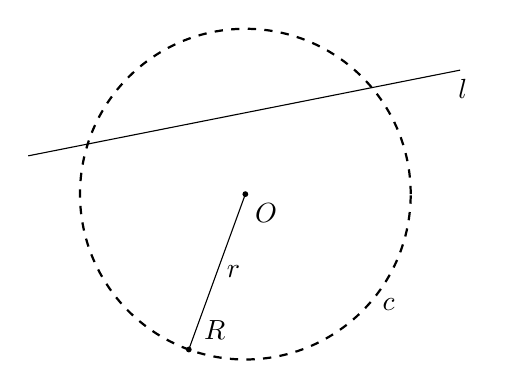
\begin{tikzpicture}[scale=.7]
\coordinate (O) at (0,0);
\node at (2.6,-2) {$c$};
\draw[thick,dashed] (O) circle[radius=3cm];
\fill (O) node[below right] {$O$} circle[radius=1.5pt];
\draw (O) -- node[right] {$r$} ++(-110:3cm) coordinate (R);
\fill (R) circle[radius=1.5pt] node[above right,xshift=2pt] {$R$};
\draw (O) +(170:4cm) -- node[below, near end,xshift=40pt,yshift=8pt] {$l$} ++(30:4.5cm);
\end{tikzpicture}
\end{center}

By Section~\ref{s.perp} it is possible to construct a perpendicular from the center of the circle $O$ to the line $l$. Label the intersection of $l$ with the perpendicular by $M$. $M$ bisects the chord $XY$, where $X, Y$ are the intersections of the line with the circle. $2s$ is the length of the chord $XY$> Note that $s,X,Y$ in the diagram are just definitions: we haven't constructed them yet.

\begin{center}
\begin{tikzpicture}[scale=.7]
\coordinate (O) at (0,0);
\node at (2.6,-2) {$c$};
\draw[thick,dashed,name path=circle] (O) circle[radius=3cm];
\fill (O) node[below right] {$O$} circle[radius=1.5pt];
\draw (O) -- node[right] {$r$} ++(-110:3cm) coordinate (R);
\fill (R) node[above right,xshift=2pt] {$R$} circle[radius=1.5pt];
\draw[name path=l] (O) ++(170:4cm) -- node[below, near end,xshift=40pt,yshift=12pt] {$l$} ++(20:8cm);
\path[name intersections={of=circle and l,by={Y,X}}];
\fill (X) node[above left] {$X$} circle[radius=1.5pt];
\fill (Y) node[above right] {$Y$} circle[radius=1.5pt];
\draw[thick,dashed] (O) -- node[below] {$r$} (X);
\path (X) -- ($(X)!.5!(Y)$) coordinate (M);
\fill (M) node[above] {$M$} circle[radius=1.5pt];
\draw[thick,dashed] (O) -- node[right] {$t$} (M);
\path (X) -- node[above] {$s$} (M);
\path (M) -- node[above] {$s$} (Y);
\draw (O) ++(170:4cm) -- ++(20:3.1cm) -- ++(-70:10pt) -- ++(20:10pt);
\end{tikzpicture}
\end{center}
$\triangle OMX$ is a right triangle, so $s^2=r^2-t^2=(r+t)(r-t)$. $r$ is given as the radius of the circle and $t$ is defined s the length of $OM$, the line segment between $O$ and $M$. By Section~\ref{s.copy} it is possible to construct a line segment of length $t$ from $O$ in the two directions $OR$ and $RO$. The result is two line segments of length $r+t,r-t$.

Section~\ref{s.root} shows how to construct a line segment of length $s=\sqrt{(r+t)(r-t)}$. By Section~\ref{s.copy} it is possible to construct line segments of length $s$ from $M$ along the given line $l$ in both directions. The other endpoints of these segments are the points of intersection of $l$ and $c$.


\section{Constructing the points of intersection of two circles}\label{s.two-circles}

\textbf{Given two circles with centers $O_1,O_2$ with radii $r_1,r_2$, it is possible to construct their points of intersection $X,Y$.}

With a straightedge it is possible to construct a line segment $O_1O_2$ that connects the two centers. Label its length $t$.

\begin{center}
\begin{tikzpicture}[scale=1.1]
\coordinate (O1) at (0,0);
\coordinate (O2) at (2.5,0);
\fill (O1) node[below left] {$O_1$} circle[radius=1.5pt];
\fill (O2) node[below right] {$O_2$} circle[radius=1.5pt];
\draw[thick,dashed,name path=circle1] (O1) circle[radius=2cm];
\draw[thick,dashed,name path=circle2] (O2) circle[radius=1.6cm];
\path [name intersections={of=circle1 and circle2,by={X,Y}}];
\draw (O1) -- node[above] {$r_1$} ++(160:2cm);
\draw (O2) -- node[above] {$r_2$} ++(30:1.6cm);
\fill (O1) ++(160:2cm) circle[radius=1.5pt];
\fill (O2) ++(30:1.6cm) circle[radius=1.5pt];
\draw (O1) -- (O2);
\node at (-1.7,1.6) {$c_1$};
\node at (3.8,1.4) {$c_2$};
\draw[<->] (0,-1) -- node[fill=white] {$t$} (2.5,-1);
\node at (6,0) {$t=O_1O_2$};
\end{tikzpicture}
\end{center}

Label by $A$ be the point of intersection of $O_1O_2$ and $XY$, and label the lengths $q=O_1A$, $x=XA$.
\begin{center}
\begin{tikzpicture}[scale=1.1]
\coordinate (O1) at (0,0);
\coordinate (O2) at (2.5,0);
\fill (O1) node[below left] {$O_1$} circle[radius=1.5pt];
\fill (O2) node[below right] {$O_2$} circle[radius=1.5pt];
\draw[thick,dashed,name path=circle1] (O1) circle[radius=2cm];
\draw[thick,dashed,name path=circle2] (O2) circle[radius=1.6cm];
\path [name intersections={of=circle1 and circle2,by={X,Y}}];
\fill (X) node[above,yshift=4pt] {$X$} circle[radius=1.5pt];
\fill (Y) node[below,yshift=-4pt] {$Y$} circle[radius=1.5pt];
\draw[thick,dashed] (O1) -- node[above,xshift=-4pt] {$r_1$} (X);
\draw[thick,dashed] (O2) -- node[above,xshift=4pt] {$r_2$} (X);
\draw[name path=oo] (O1) -- (O2);
\node at (-1.7,1.6) {$c_1$};
\node at (3.8,1.4) {$c_2$};
\draw[name path=xy] (X) -- (Y);
\path[name intersections={of=xy and oo,by={A}}];
\fill (A) node[below left] {$A$} circle[radius=1.5pt];
\path (O1) -- node[below,xshift=-2pt] {$q$} (A);
\path (X) -- node[left,yshift=-2pt] {$x$} (A);
\draw[<->] (0,-1) -- node[fill=white] {$t$} (2.5,-1);
\node at (6,.5) {$t=O_1O_2$};
\node at (6,0) {$q=O_1A$};
\node at (6,-.5) {$x=XA$};
\end{tikzpicture}
\end{center}
Note that we have not constructed $A$, but if we succeed in constructing the lengths $q,x$, by Section~\ref{s.copy} we can construct $A$ at length $q$ from $O_1$ in the direction $O_1O_2$. By Section~\ref{s.perp} perpendicular to $O_1O_2$ at $A$ can be constructed and again by Section~\ref{s.copy} it is possible to construct line segments of length $x$ from $A$ is both directions along the perpendicular. The other endpoints $X,Y$ of the these sections are  the points of intersection of the circles.

\textbf{Constructing the length $q$:} Define $d=\sqrt{r_1^2+t^2}$, the hypotenuse of a right triangle. It can be constructed from $r_1,t$, the known lengths of the other two sides. On any line construct a line segment $RS$ of length $r_1$, then a perpendicular to $RS$ throught $R$, and finally, a line segment $RT$ of length $t$ through $R$ on the perpendicular. The length of the hypotenuse $ST$ is $d$. This right triangle can be constructed anywhere in the plane, not necessarily near the circles.

By the law of cosines for $\triangle O_1O_2X$:
\erh{12pt}
\begin{equationarray*}{rcl}
r_2^2 &=& r_1^2 + t^2 - 2r_1t\cos\angle XO_1O_2\\
&=& r_1^2 + t^2 - 2tq\\
q&=&\disfrac{(d+r_2)(d-r_2)}{2t}\,.
\end{equationarray*}
By Section~\ref{s.copy} these lengths can be constructed and by Section~\ref{s.relative} $q$ can be constructed from $d+r_2,d-r_2,2t$.

\textbf{Constructing the length x:} $\triangle AO_1X$ is a right triangle, so $x=\sqrt{r_1^2-q^2}=\sqrt{(r_1+q)(r_1-q)}$. By Section~\ref{s.copy} $h =r_1+ q,k= r_1 - q$ can be constructed, as can $x=\sqrt{hk}$ by Section~\ref{s.root}.

